\documentclass[conference]{IEEEtran}
\IEEEoverridecommandlockouts
% The preceding line is only needed to identify funding in the first footnote. If that is unneeded, please comment it out.
\usepackage{cite}
\usepackage{amsmath,amssymb,amsfonts}
\usepackage{algorithmic}
\usepackage{graphicx}
\usepackage{textcomp}
\usepackage{xcolor}
\def\BibTeX{{\rm B\kern-.05em{\sc i\kern-.025em b}\kern-.08em
    T\kern-.1667em\lower.7ex\hbox{E}\kern-.125emX}}
\begin{document}

\title{A Real-time Clustering Scheme using Coordinate Density for 3D Indoor Localization\\
    \thanks{}}

\author{\IEEEauthorblockN{\textsuperscript{} Ho Chul Lee}
    \IEEEauthorblockA{\textit{Dept. of Computer Engineering} \\
        \textit{Tongmyong University}\\
        Busan, Republic of Korea \\
        calmtot@gmail.com}
    \and
    \IEEEauthorblockN{\textsuperscript{} Dong Myung Lee}
    \IEEEauthorblockA{\textit{Dept. of Computer Engineering} \\
        \textit{Tongmyong University}\\
        Busan, Republic of Korea \\
        dmlee@tu.ac.kr}
}

\maketitle

\begin{abstract}
    A demand for indoor localization technology in the field of automation is growing very rapidly. Typical examples include logistics automation and construction safety management and so on. In general, the trilateration is used to indoor localization, the performance of the sensed data is greatly affected by the surrounding radio frequency and obstacle environments, so there is a lot of errors in the measured data. In this paper, we proposed a real-time clustering scheme using coordinate density to improve this problems in 3D indoor localization. It was confirmed that the proposed clustering scheme can significantly reduce the localization error in indoor obstacle environments.
\end{abstract}


\begin{IEEEkeywords}
    Sensor, 3D localization, trilateration, clustering, coordinate density
\end{IEEEkeywords}

\section{Introduction}
As labor costs become more expensive and industries become more complex, the number of skilled workers is shrinking. In this trend, automation has long played an important role in manufacturing \cite{b1}. Among technologies for automation industry, localization can be applied in many industrial location based services (LBS). \cite{b2}.

However, since global positioning system (GPS) signals cannot be used in indoor localization, various technologies such as Wi-Fi, Bluetooth, RFID, ultra wide band (UWB), infrared and ultrasonic are utilized \cite{b3}. However, in this case, it is impossible to provide localization performance at the GPS level. In the case of indoor localization, errors occur in measurement data because most of them are greatly influenced by indoor environments. If these errors can be eliminated, indoor localization accuracy can be greatly improved. According to \cite{b4,b5,b6}, it can be confirmed that the localization accuracy is improved using a clustering scheme based on measured coordinate densities in 2D indoor localization.

In this paper, we first introduced the multi-triangulation using radio anchors and tags. Then, a clustering scheme and a minimum distance algorithm were proposed to remove the error of the measured coordinates for 3D indoor localization. The performance of the proposed real-time clustering scheme was evaluated through experiments using the developed test bed tool. Finally, conclusions and future studies are summarized.

The clustering scheme first calculates the total estimated coordinates of a tag using trilateration based on four tags. Then, based on the allowable distance error, all estimated coordinates are classified into several clustering regions. Therefore, each clustering region has different estimated coordinate densities. If the calculated regions have the same coordinate density, the region with a high coordinate density weight is selected using the minimum distance algorithm. Therefore, the average value of the estimated tag coordinates in the selected region becomes the final coordinate of the tag.


\section{System Architecture}

\subsection{Key Considerations for 3D indoor positioning}
In order to perform trilateration in indoor localization, at least three anchors are basically required. If any one of the three anchors does not work, the localization fails. There are many causes of anchor failure, mainly errors occur when there are obstacles between the tag and the anchor or the anchor's power supply is faulty. These errors often occur indoors with many obstacles.

The more frequent these errors occur, the more unstable the indoor localization performance becomes \cite{b7}. In this case, the localization failure can be improved by adding an anchor. That is, even if a problem occurs in any one anchor, the probability of positioning is higher than when no anchor is added\cite{b8}.

\subsection{Multiple trilateration using four anchors}
The proposed scheme first collects the coordinates of each anchor and the distance value between tag. Then, the coordinates of the tag are calculated using trilateration. As shown in Fig. \ref{fig1}, the number of coordinates that can be obtained through trilateration using three spheres is two. Therefore, as shown in Fig. \ref{fig2}, since the total number of anchor is four, the number of collectable coordinates is eight as in Eq. (\ref{eq1}).

\begin{equation}
    2\binom{4}{3} = 2\frac{4!}{(4-3)!3!}=8\label{eq1}
\end{equation}

\begin{figure}[htbp]
    \centerline{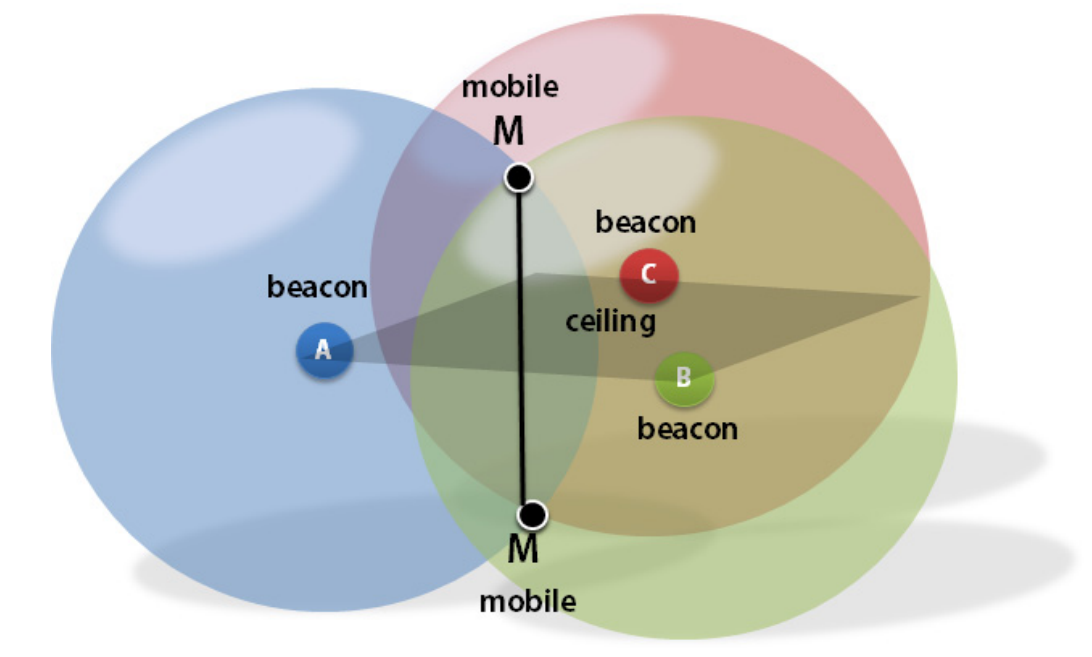
\includegraphics[width=0.8\columnwidth]{fig2.png}}
    \caption{Calculation of 3D coordinates based on 3 spheres.}
    \label{fig1}
\end{figure}

\begin{figure}[htbp]
    \centerline{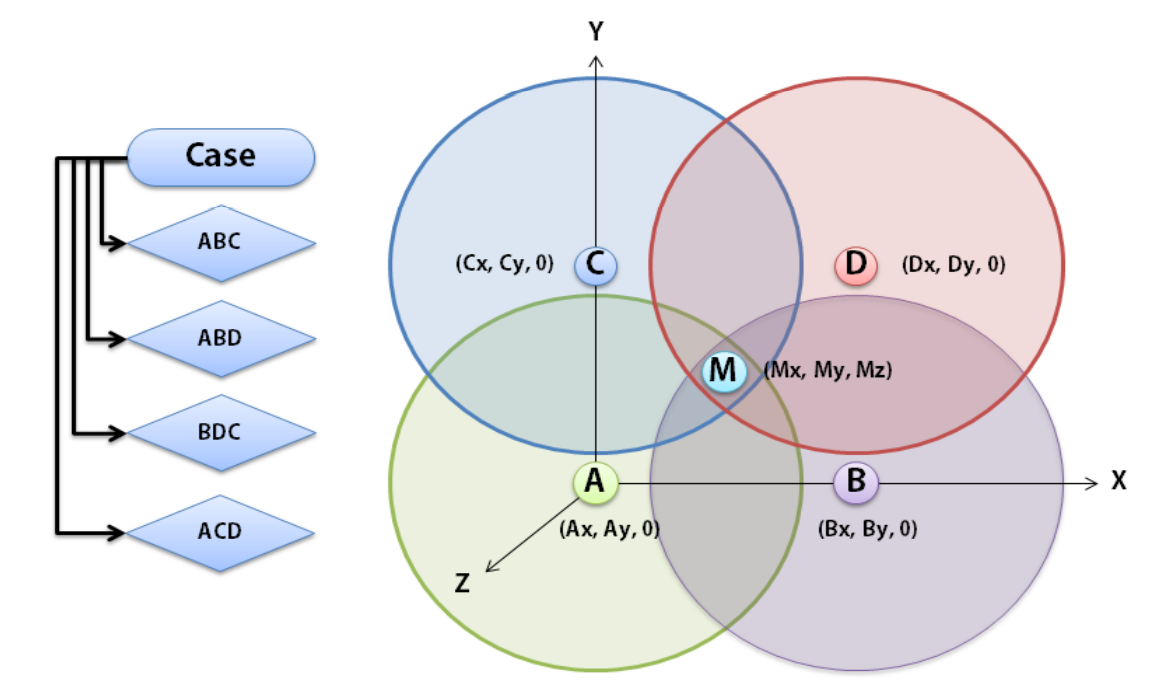
\includegraphics[width=0.9\columnwidth]{fig1.png}}
    \caption{Coordinates calculation of tag node using 4 anchors.}
    \label{fig2}
\end{figure}


\subsection{Clustering scheme using the density of coordinates}
Trilateration with four anchors obtains multiple tag coordinates. However, as shown in Fig. \ref{fig1}, one of the two coordinates is far from the actual tag location. Therefore, if the proposed clustering scheme using coordinate density is used, it is possible to remove the coordinates of the tag far from the actual tag coordinate. Therefore, it is possible to improve the accuracy of indoor localization by using only the coordinates closest to the actual tag coordinate.

When measuring the distance between the anchor and tag in indoors, an error can be occurred in the distance. For example, when positioning a tag using four anchors, an error may occur in one or more of four anchors due to an obstacle between the tag and the anchor. The proposed clustering scheme can quickly remove these errors. The distance between two coordinates is calculated by combining the two coordinates.The number of branches of the calculated distance is extracted to 28 pairs as in Eq. (\ref{eq2}). The clustering scheme finds the highest density among the 8 tag coordinates calculated when trilateration is performed 4 times.

\begin{equation}
    \binom{8}{2} = \frac{8!}{(8-2)!2!}=28\label{eq2}
\end{equation}

As shown in Fig. \ref{fig3}, the 3D indoor localization scheme determines the tag coordinates, and then selects a pair within allowable distance error. The error was assumed to 1 m in this paper. The proposed scheme selects the region with the largest number of pairs connected between nodes among the selected coordinates. It then averages the selected coordinates to determine one estimated tag coordinate.



\begin{figure}[htbp]
    \centerline{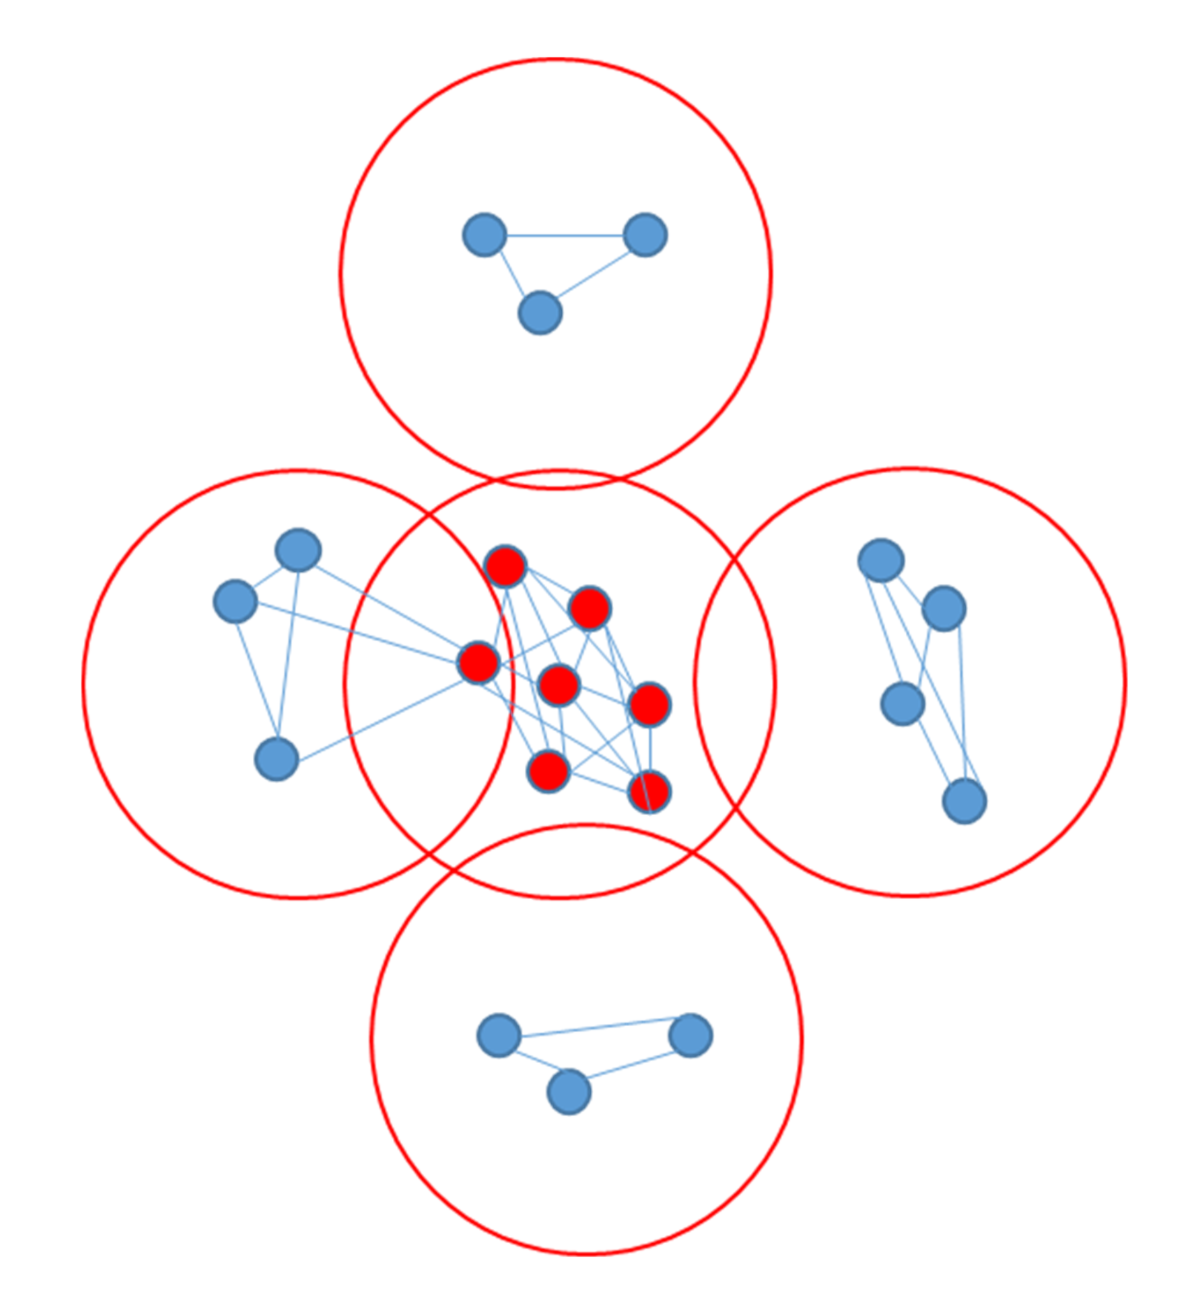
\includegraphics[width=0.7\columnwidth]{fig3.png}}
    \caption{Clustering scheme using density of coordinates.}
    \label{fig3}
\end{figure}


As shown in Fig \ref{fig4}, one coordinate of the tag is determined as the average of the coordinate sets of the minimum distance. For example, if there are 4 clustering regions and each density is [4, 4, 2, 3], the tag has 2 coordinates because region 1 and region 2 have the same density. The proposed real-time clustering scheme uses the minimum distance algorithm to select a region with a high average coordinate weight, that is, a high coordinate density.


\begin{figure}[htbp]
    \centerline{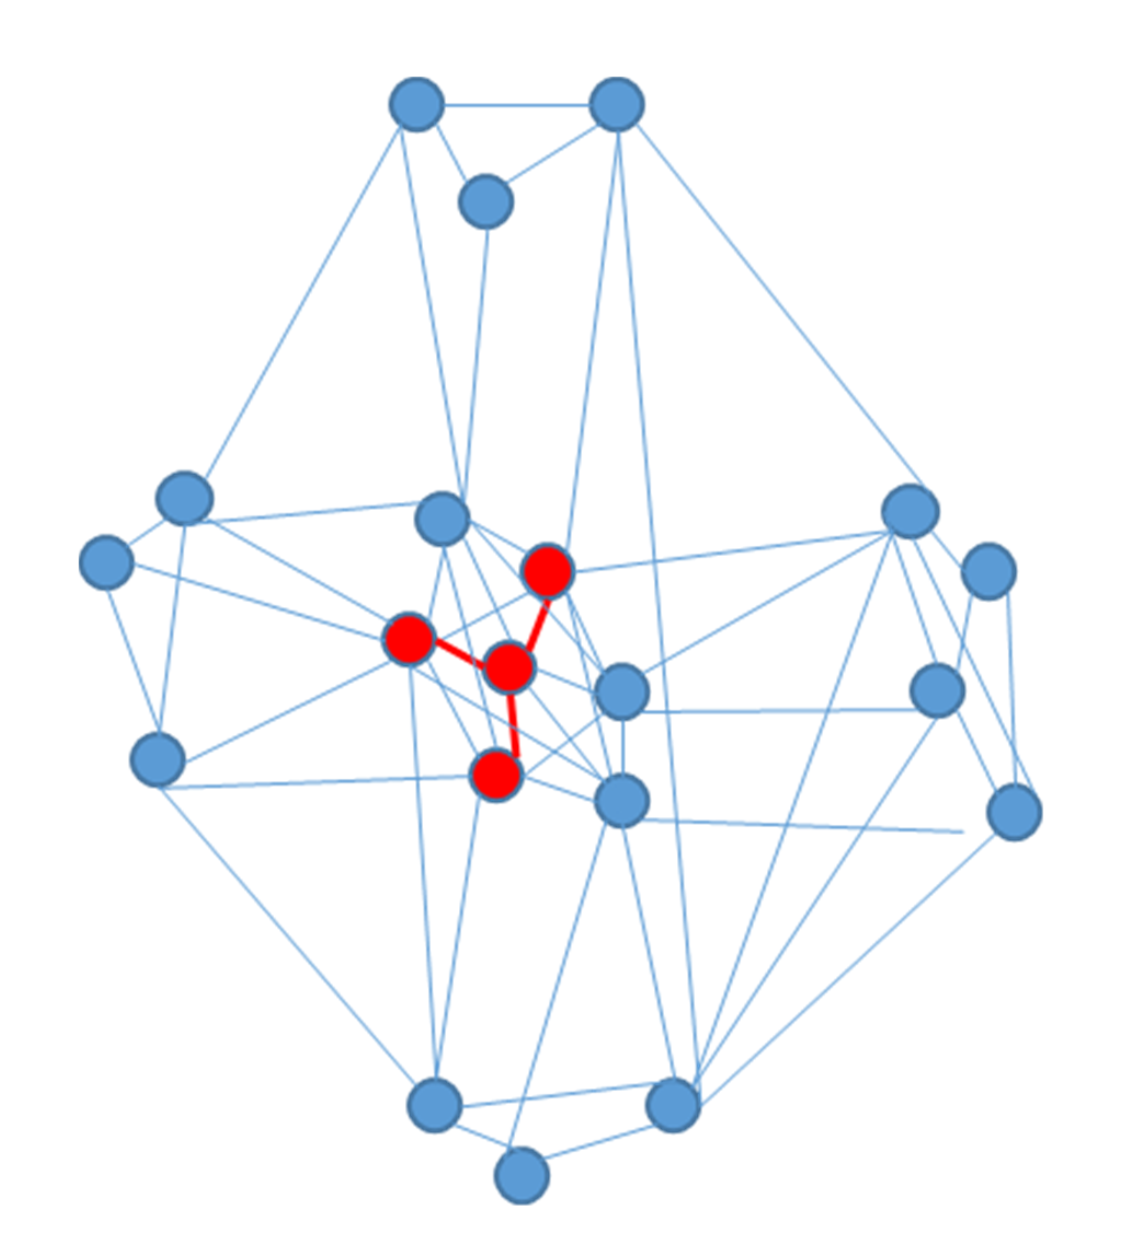
\includegraphics[width=0.5\columnwidth]{fig4.png}}
    \caption{Minimum distance method on same density of coordinates.}
    \label{fig4}
\end{figure}

\section{Experiments and Result Analysis}
\subsection{Experiments}

As shown in Fig. \ref{fig5}, the developed test bed tool for the performance experiment of indoor localization consists of 4 anchors, 1 tag, and 1 gateway, and it is a tool that can execute an experiment of indoor localization in real time. The developed test bed tool was developed with UWB radio modules, and the distance between tag and anchor was measured using two way ranging (TWR).

\begin{figure}[htbp]
    \centerline{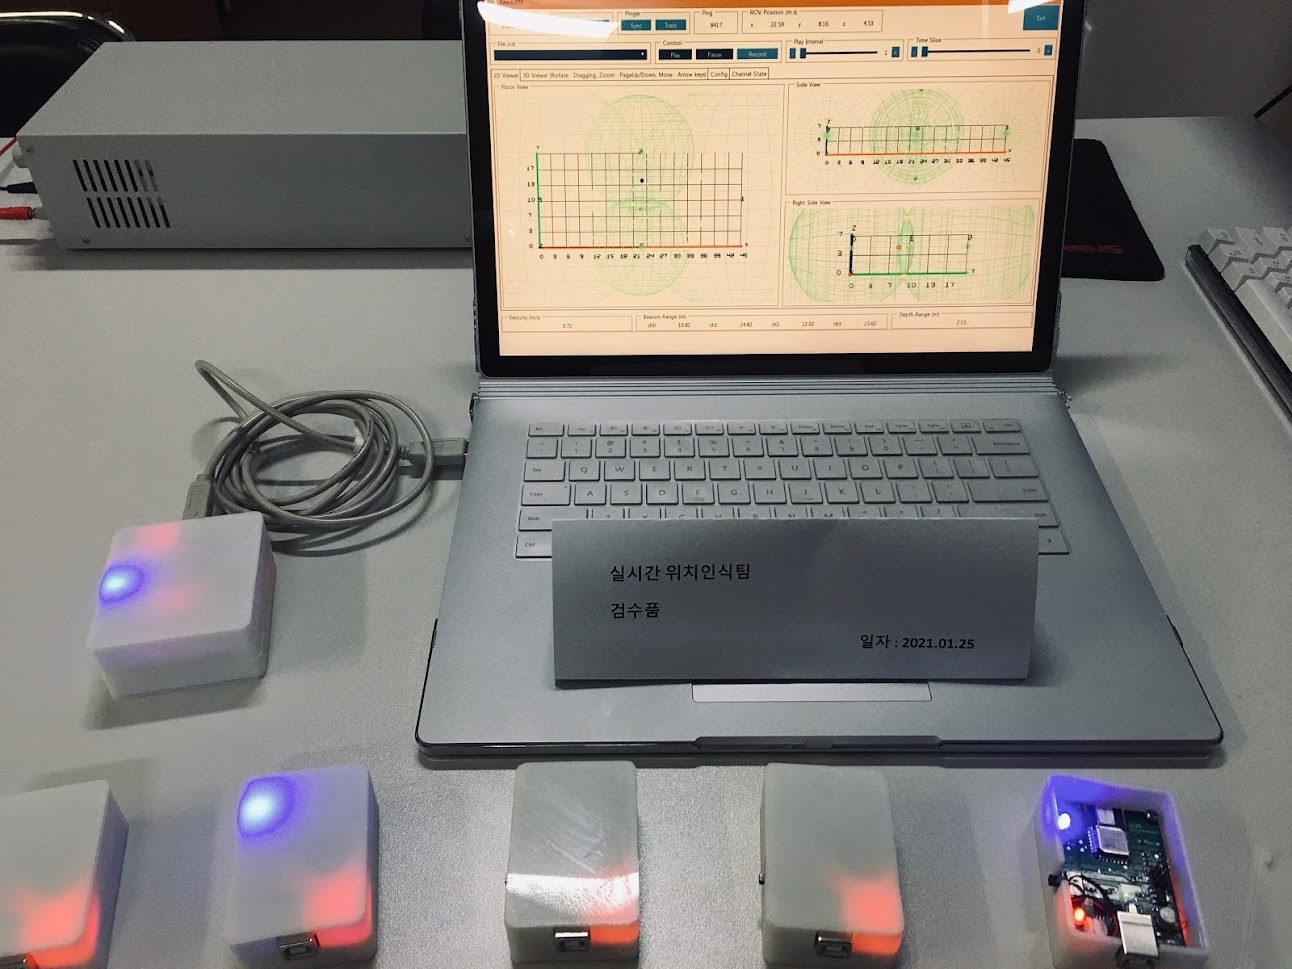
\includegraphics[width=0.8\columnwidth]{fig10.jpg}}
    \caption{Test bed for 3D indoor localization.}
    \label{fig5}
\end{figure}


As shown in Fig. \ref{fig6}, the developed test bed for indoor localization performance tracks the the tag coordinates when it receives a signal from the gateway. The operation process of the test bed consists of a top view, a side view, a front view, and a 3D image screen in Fig. 6. The screen on the right shows the moving path of the tag in real time as a graph, and the 3D coordinates and speed of the moving tag are displayed in time series on the graph.

The developed test bed can also enable or disable the proposed clustering scheme and minimum distance algorithm. Using these functions, the performance of the proposed algorithm can be evaluated.

\begin{figure}[htbp]
    \centerline{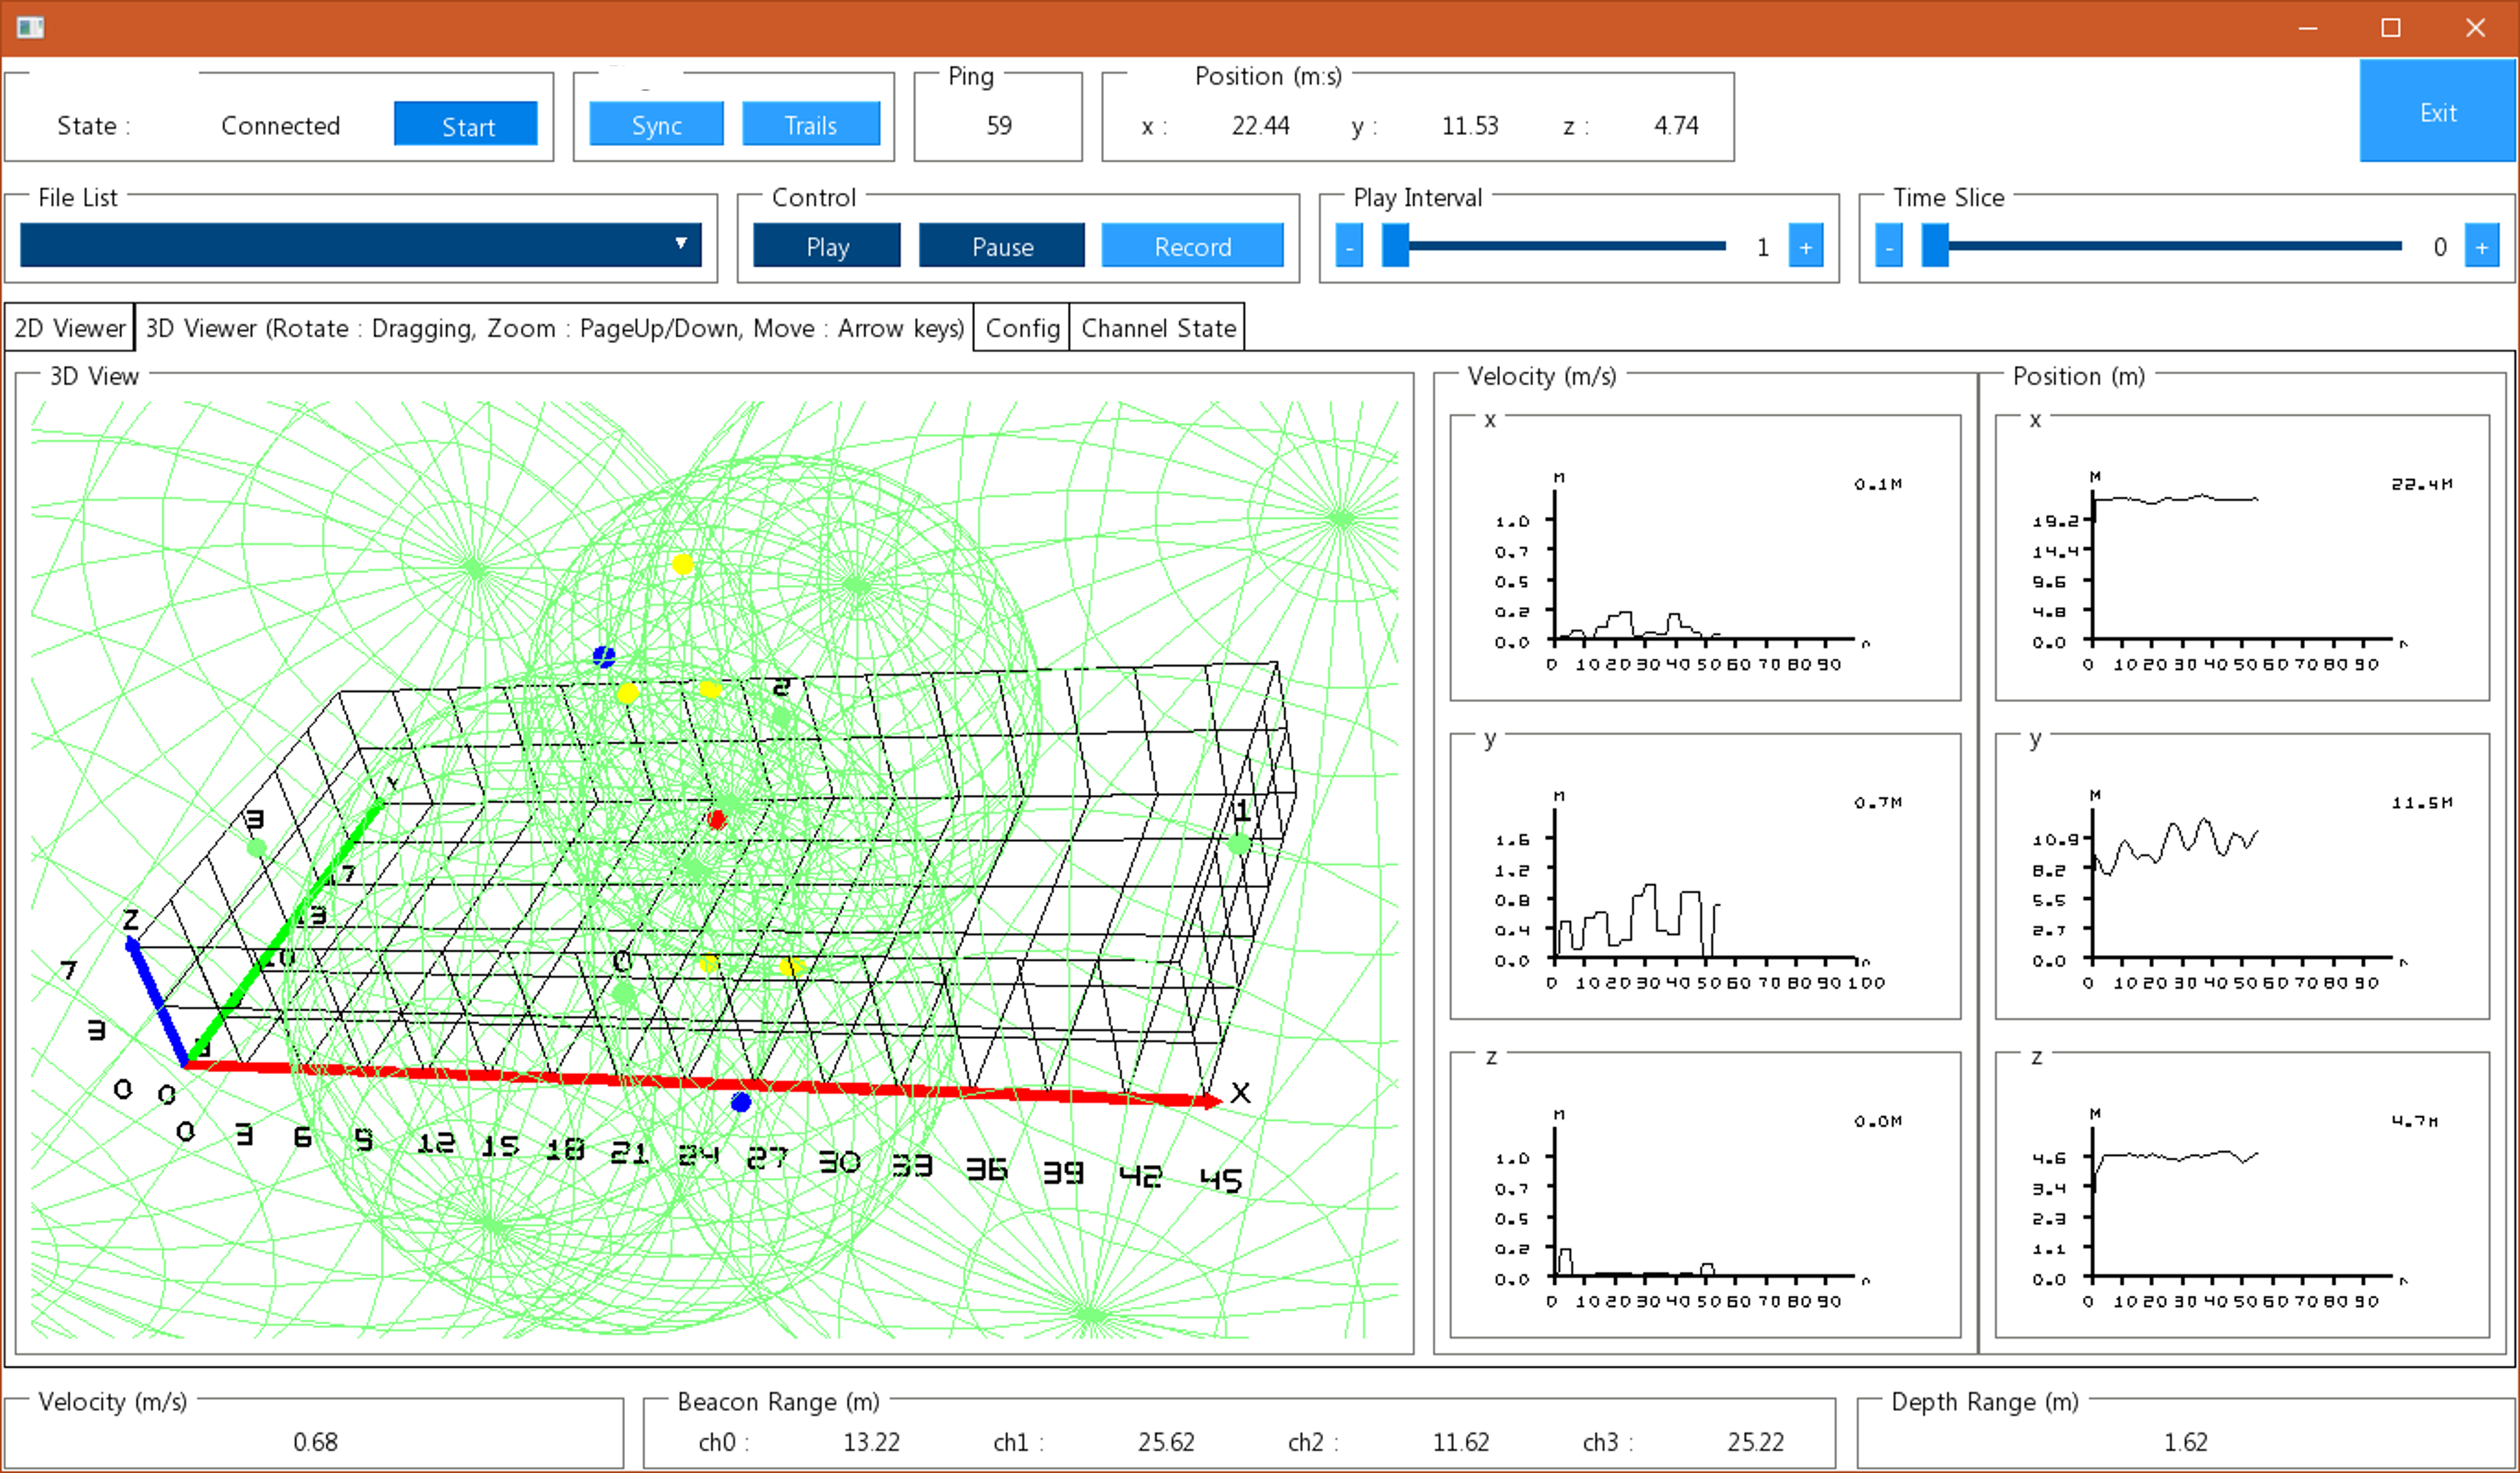
\includegraphics[width=0.9\columnwidth]{fig5.png}}
    \caption{Operation process in developed test bed for indoor positioning performance.}
    \label{fig6}
\end{figure}



The moving process of the tag is monitored in real time in 3D space as shown in Fig. \ref{fig7} in the developed test bed. The x-y coordinates of the tag are shown in the top view, the y-z coordinates in the side view, and the x-z coordinates in the front view, respectively. The distance between tag and anchor is displayed as a 3D sphere. The  error in the measured distance can be also visually seen using a 3D sphere. In addition, the moving path of tag using the proposed clustering scheme is displayed in 2D with a red line as shown in Fig. \ref{fig8}, and can be evaluated visually.

The test bed can track the tag movement in real time in 3D space as shown in Fig. \ref{fig9} in 3D from various angles using visualization.


\begin{figure}[htbp]
    \centerline{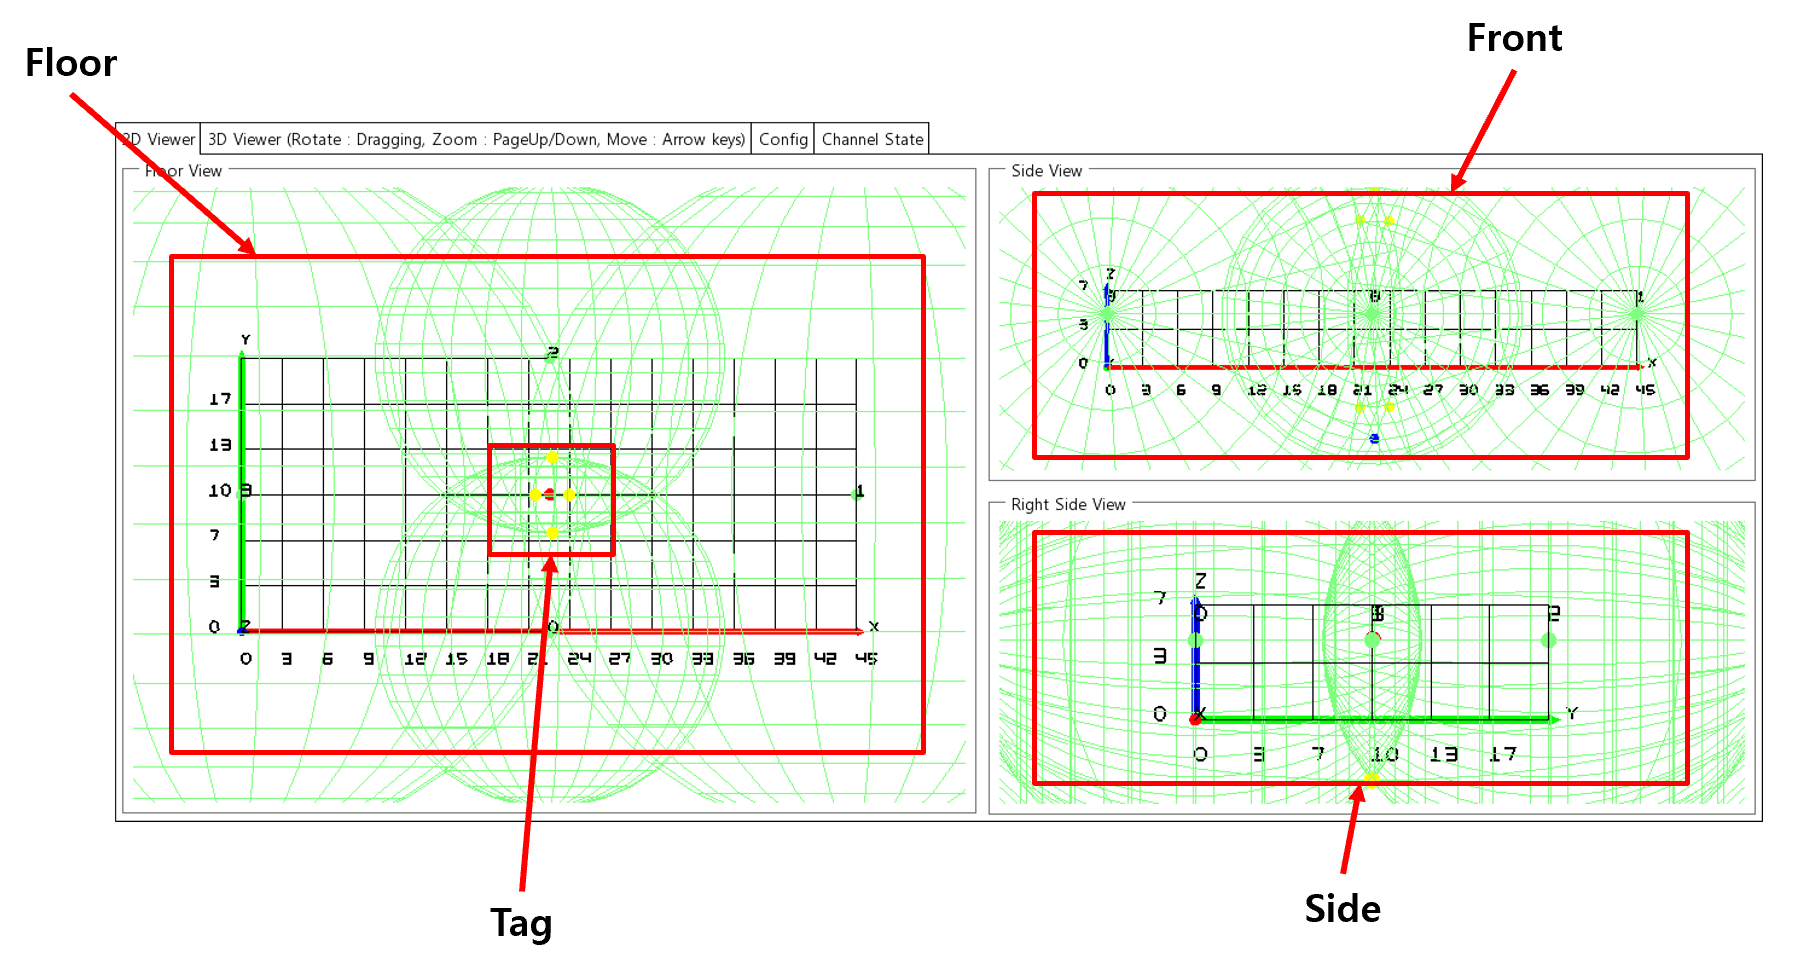
\includegraphics[width=1.0\columnwidth]{fig6.png}}
    \caption{Real-time monitoring of tag movement.}
    \label{fig7}
\end{figure}


\begin{figure}[htbp]
    \centerline{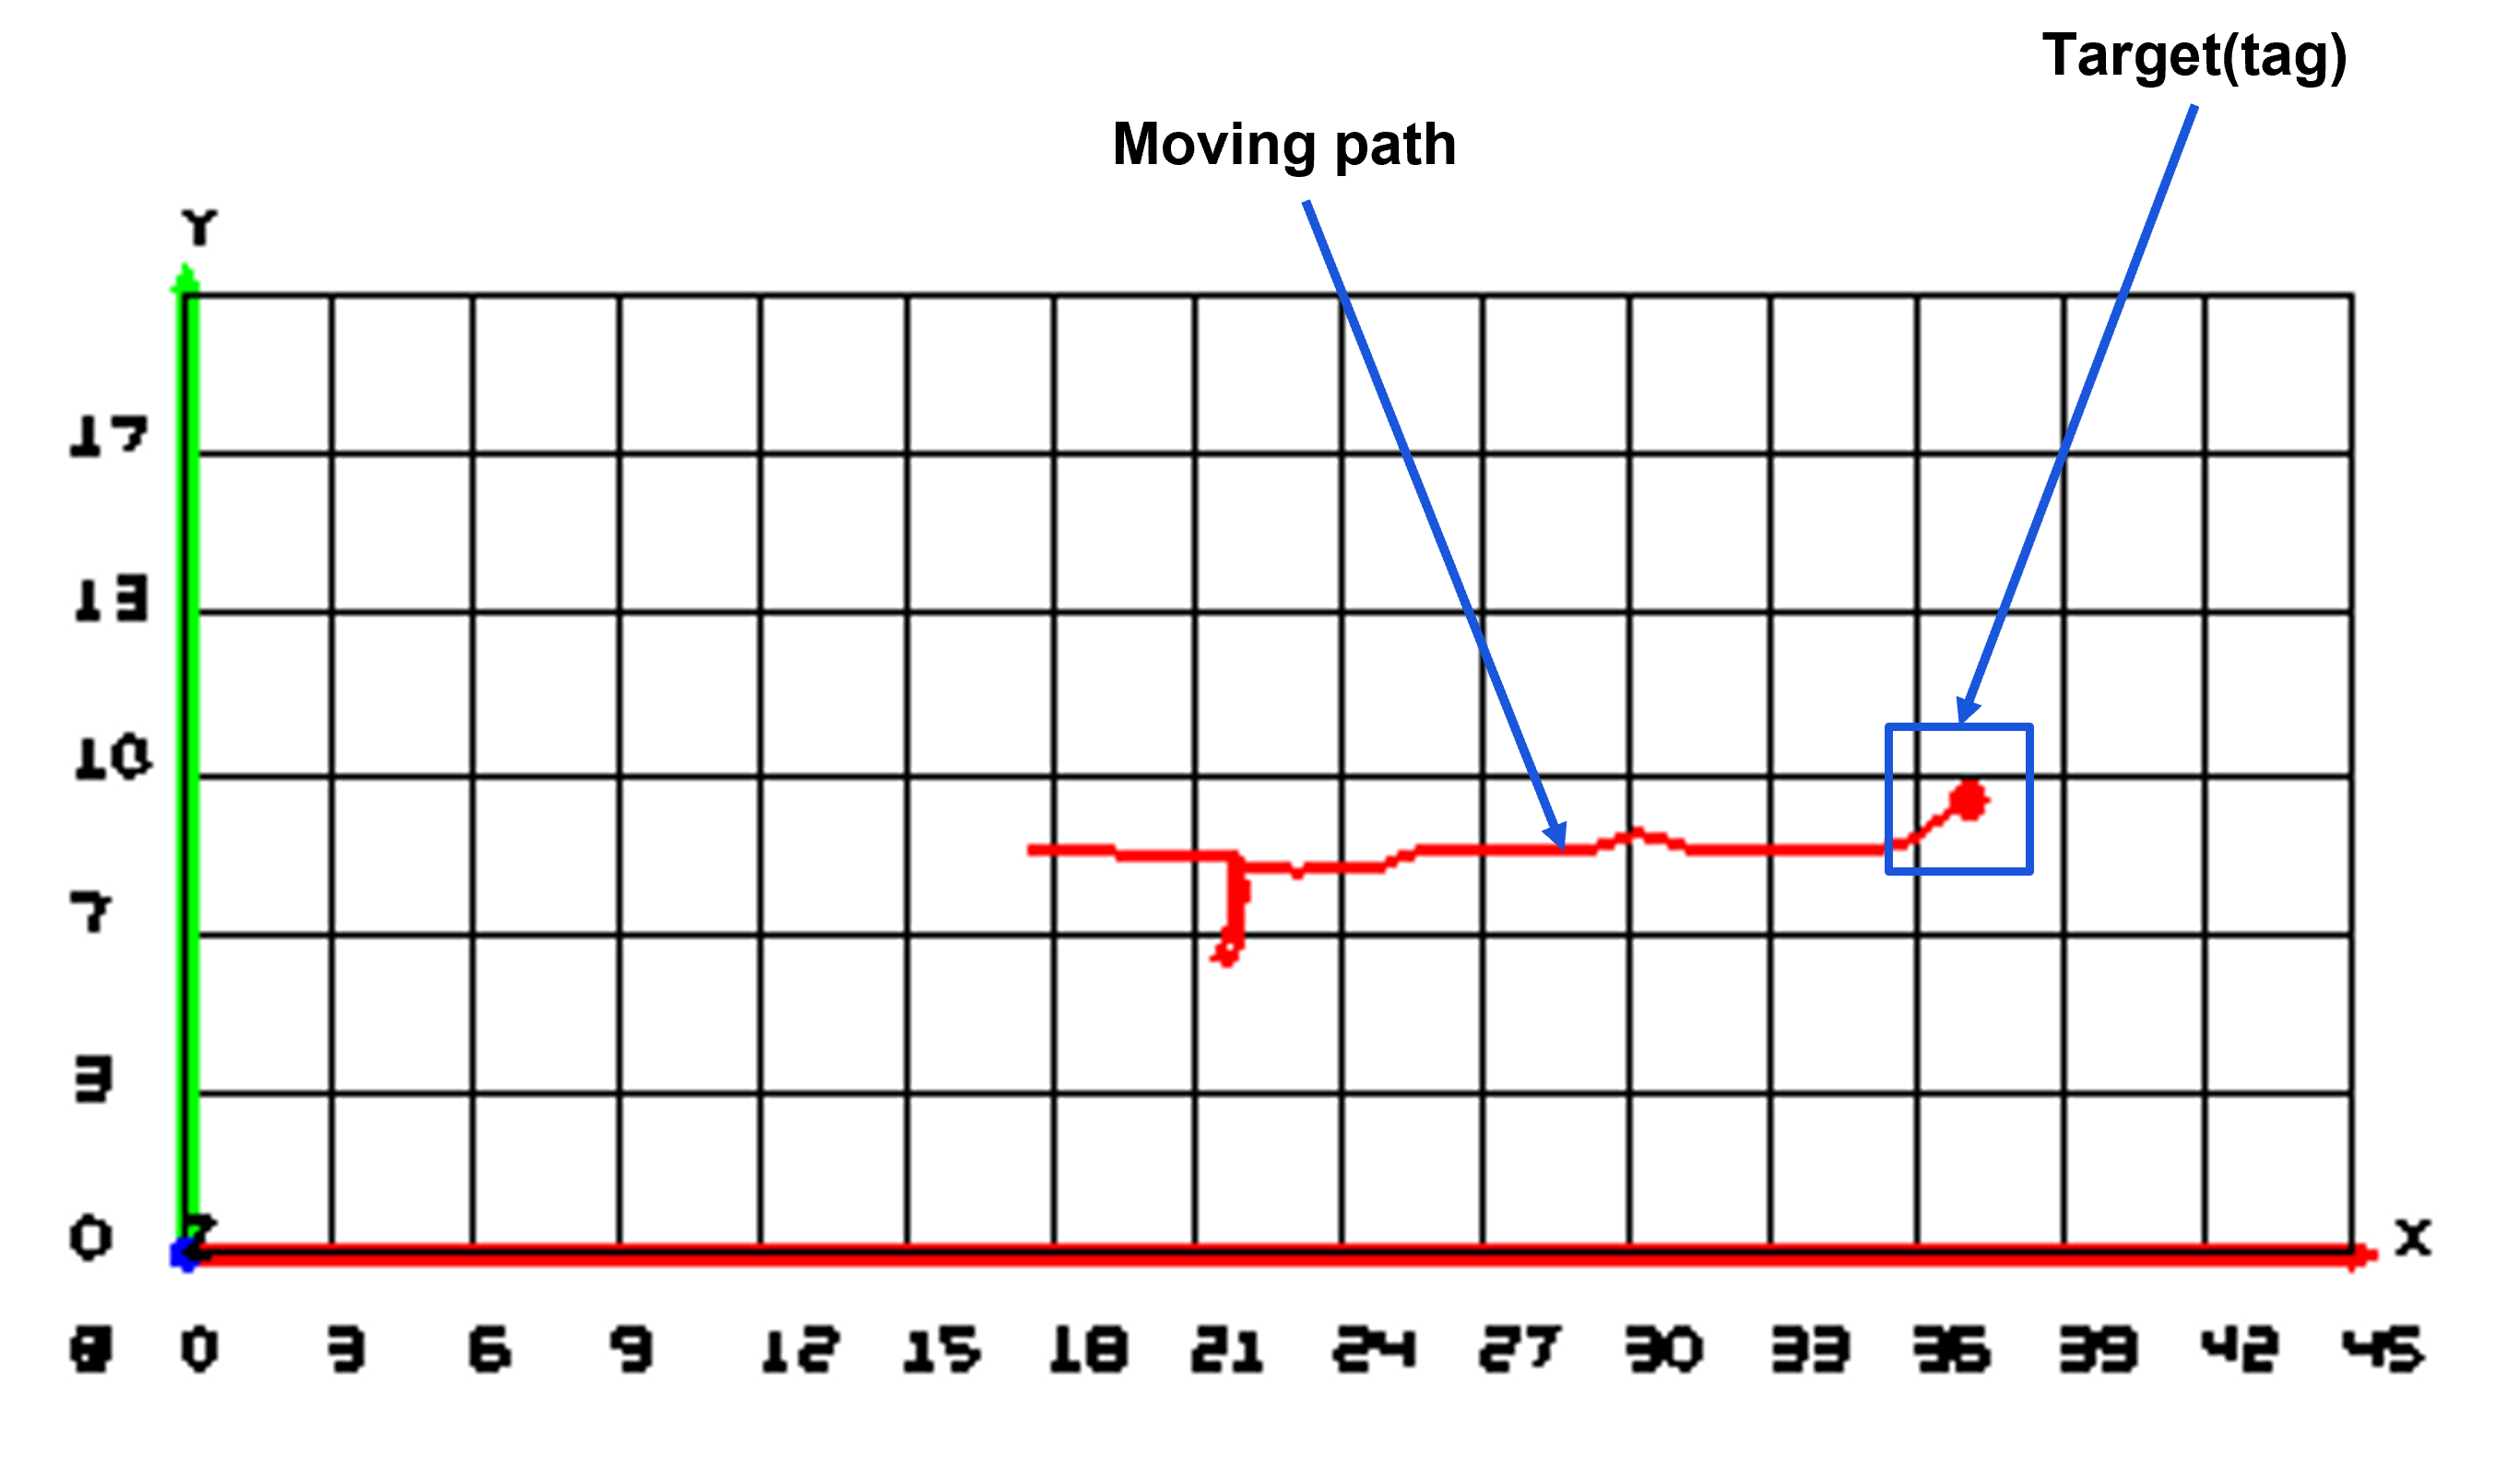
\includegraphics[width=0.9\columnwidth]{fig7.png}}
    \caption{Real-time path tracking of tag movement.}
    \label{fig8}
\end{figure}


\begin{figure}[htbp]
    \centerline{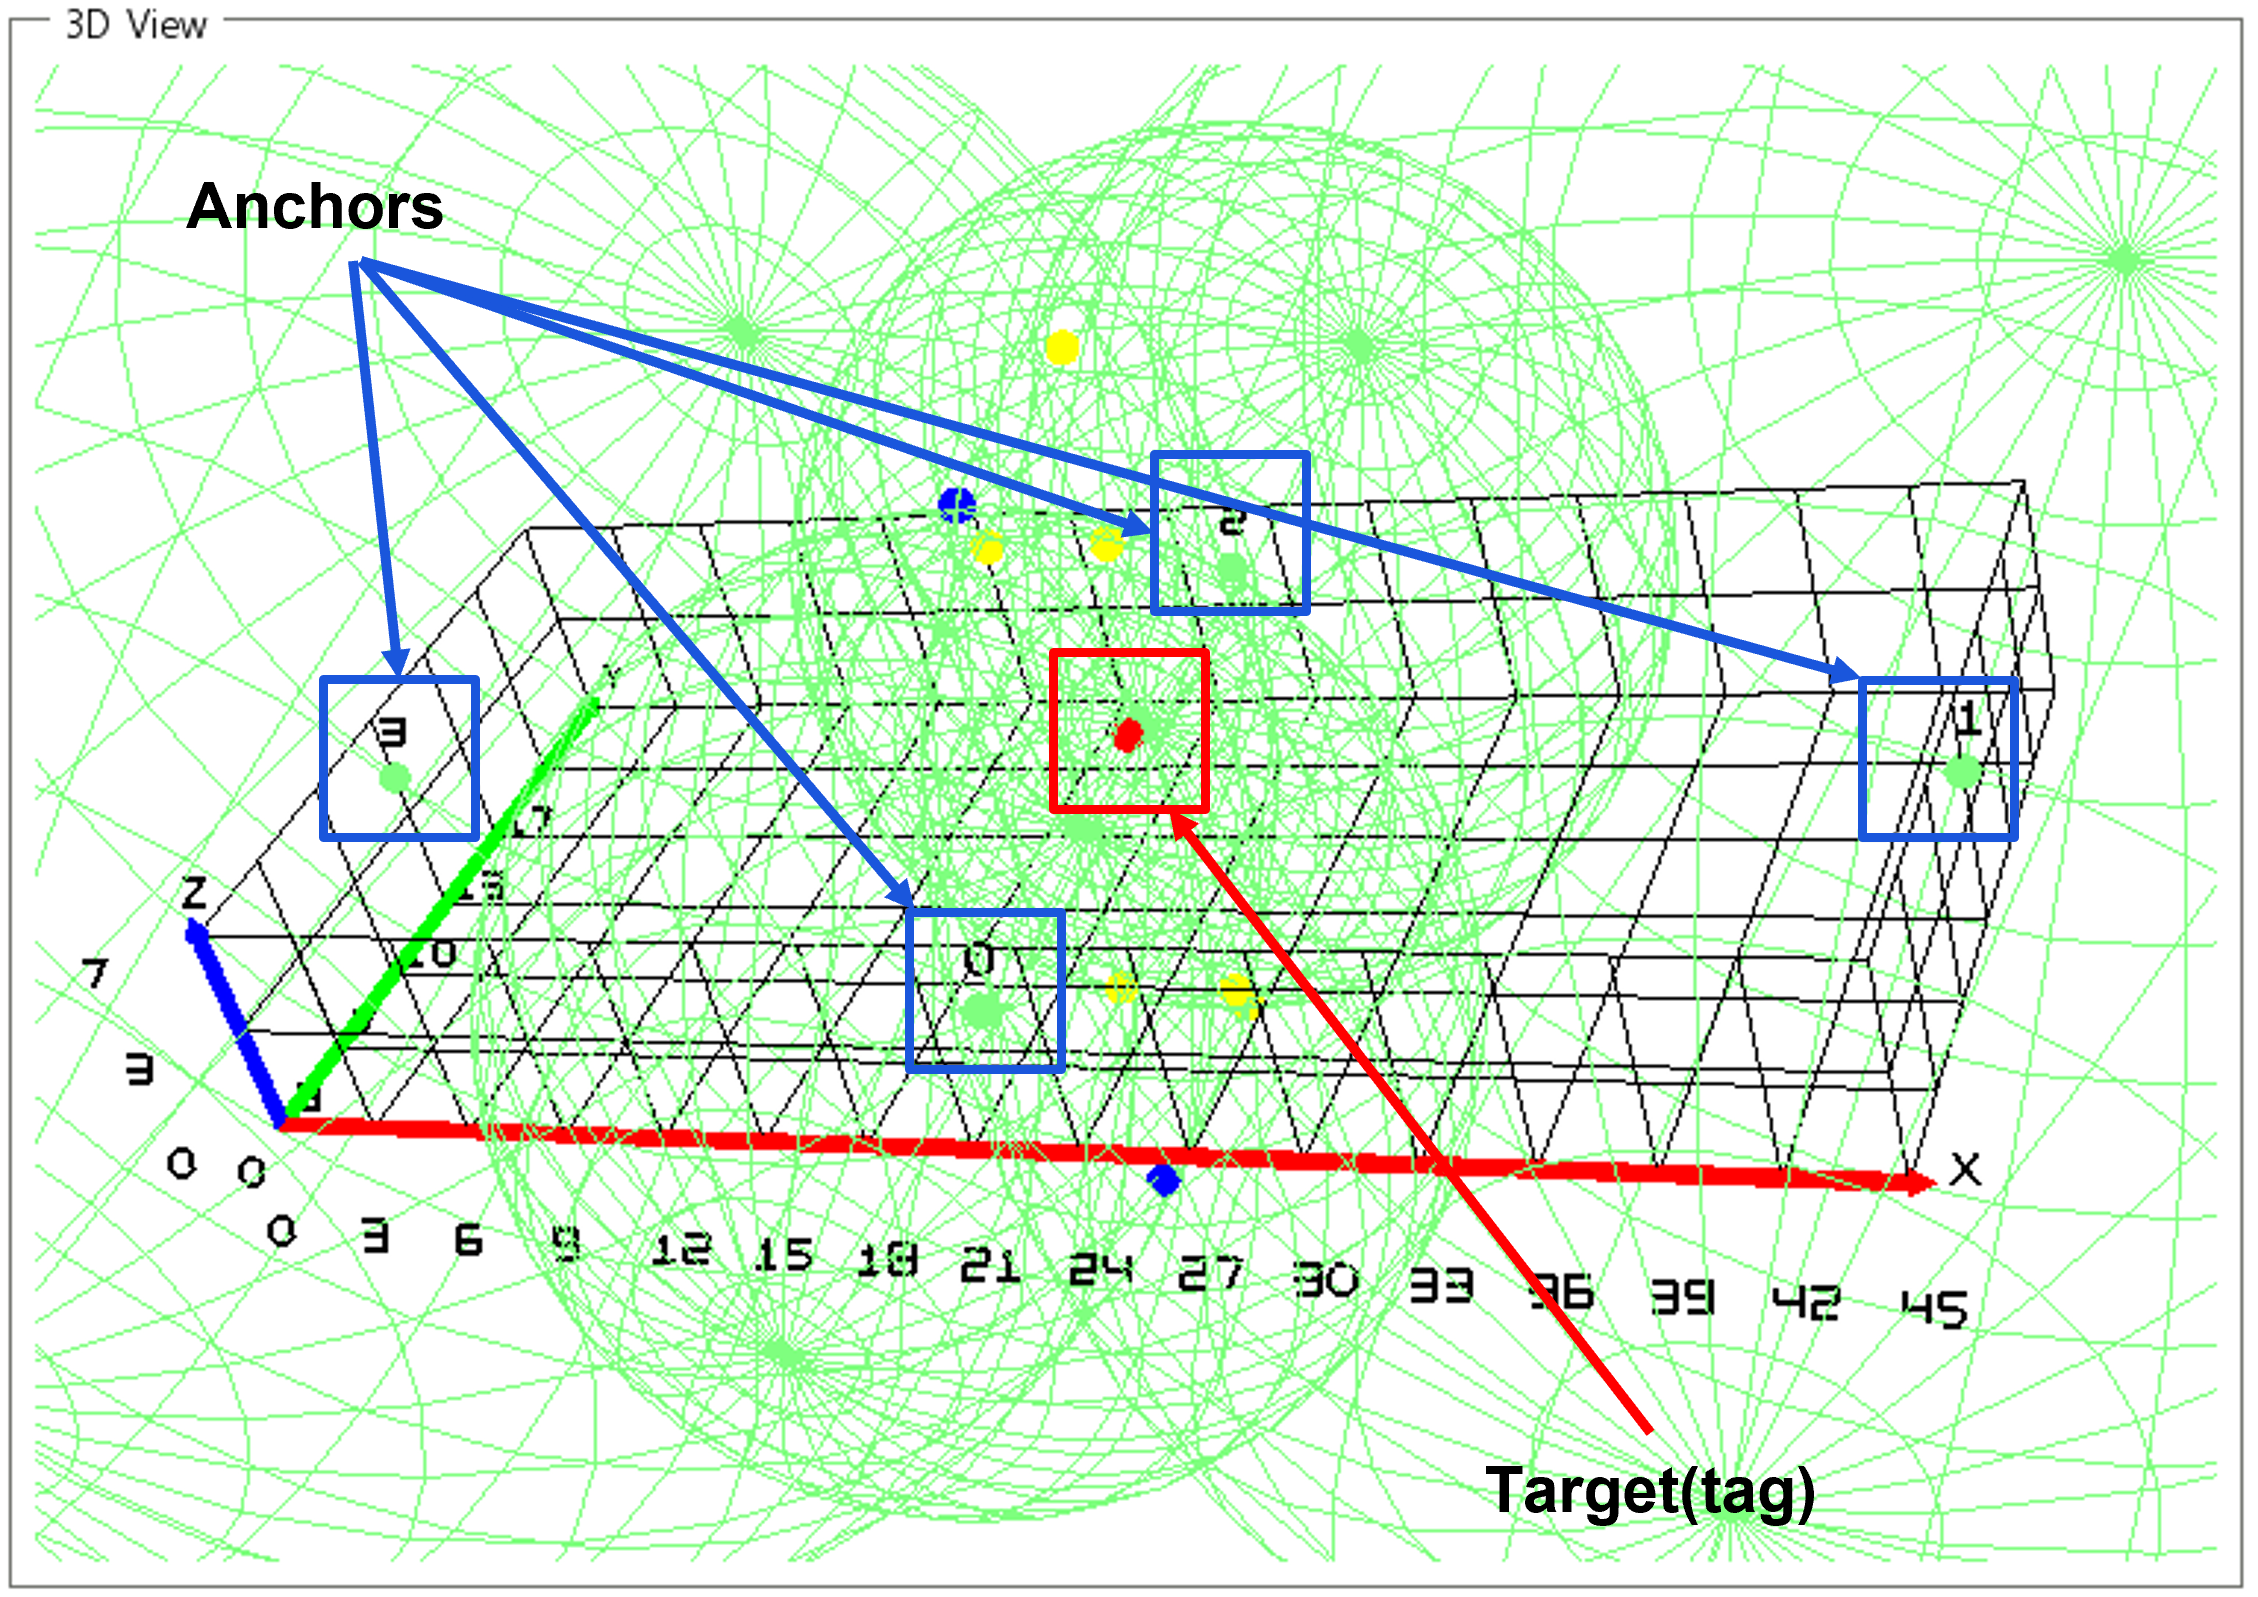
\includegraphics[width=0.8\columnwidth]{fig8.png}}
    \caption{3D visualization of tag movement on multiple angles.}
    \label{fig9}
\end{figure}


The speed and coordinate of tag is visually displayed as a graph on each coordinate axis, as shown in Fig. \ref{fig10}, and is updated in real time. Using these graphs, the performance of the proposed clustering scheme using coordinate density can be visually evaluated.

\begin{figure}[htbp]
    \centerline{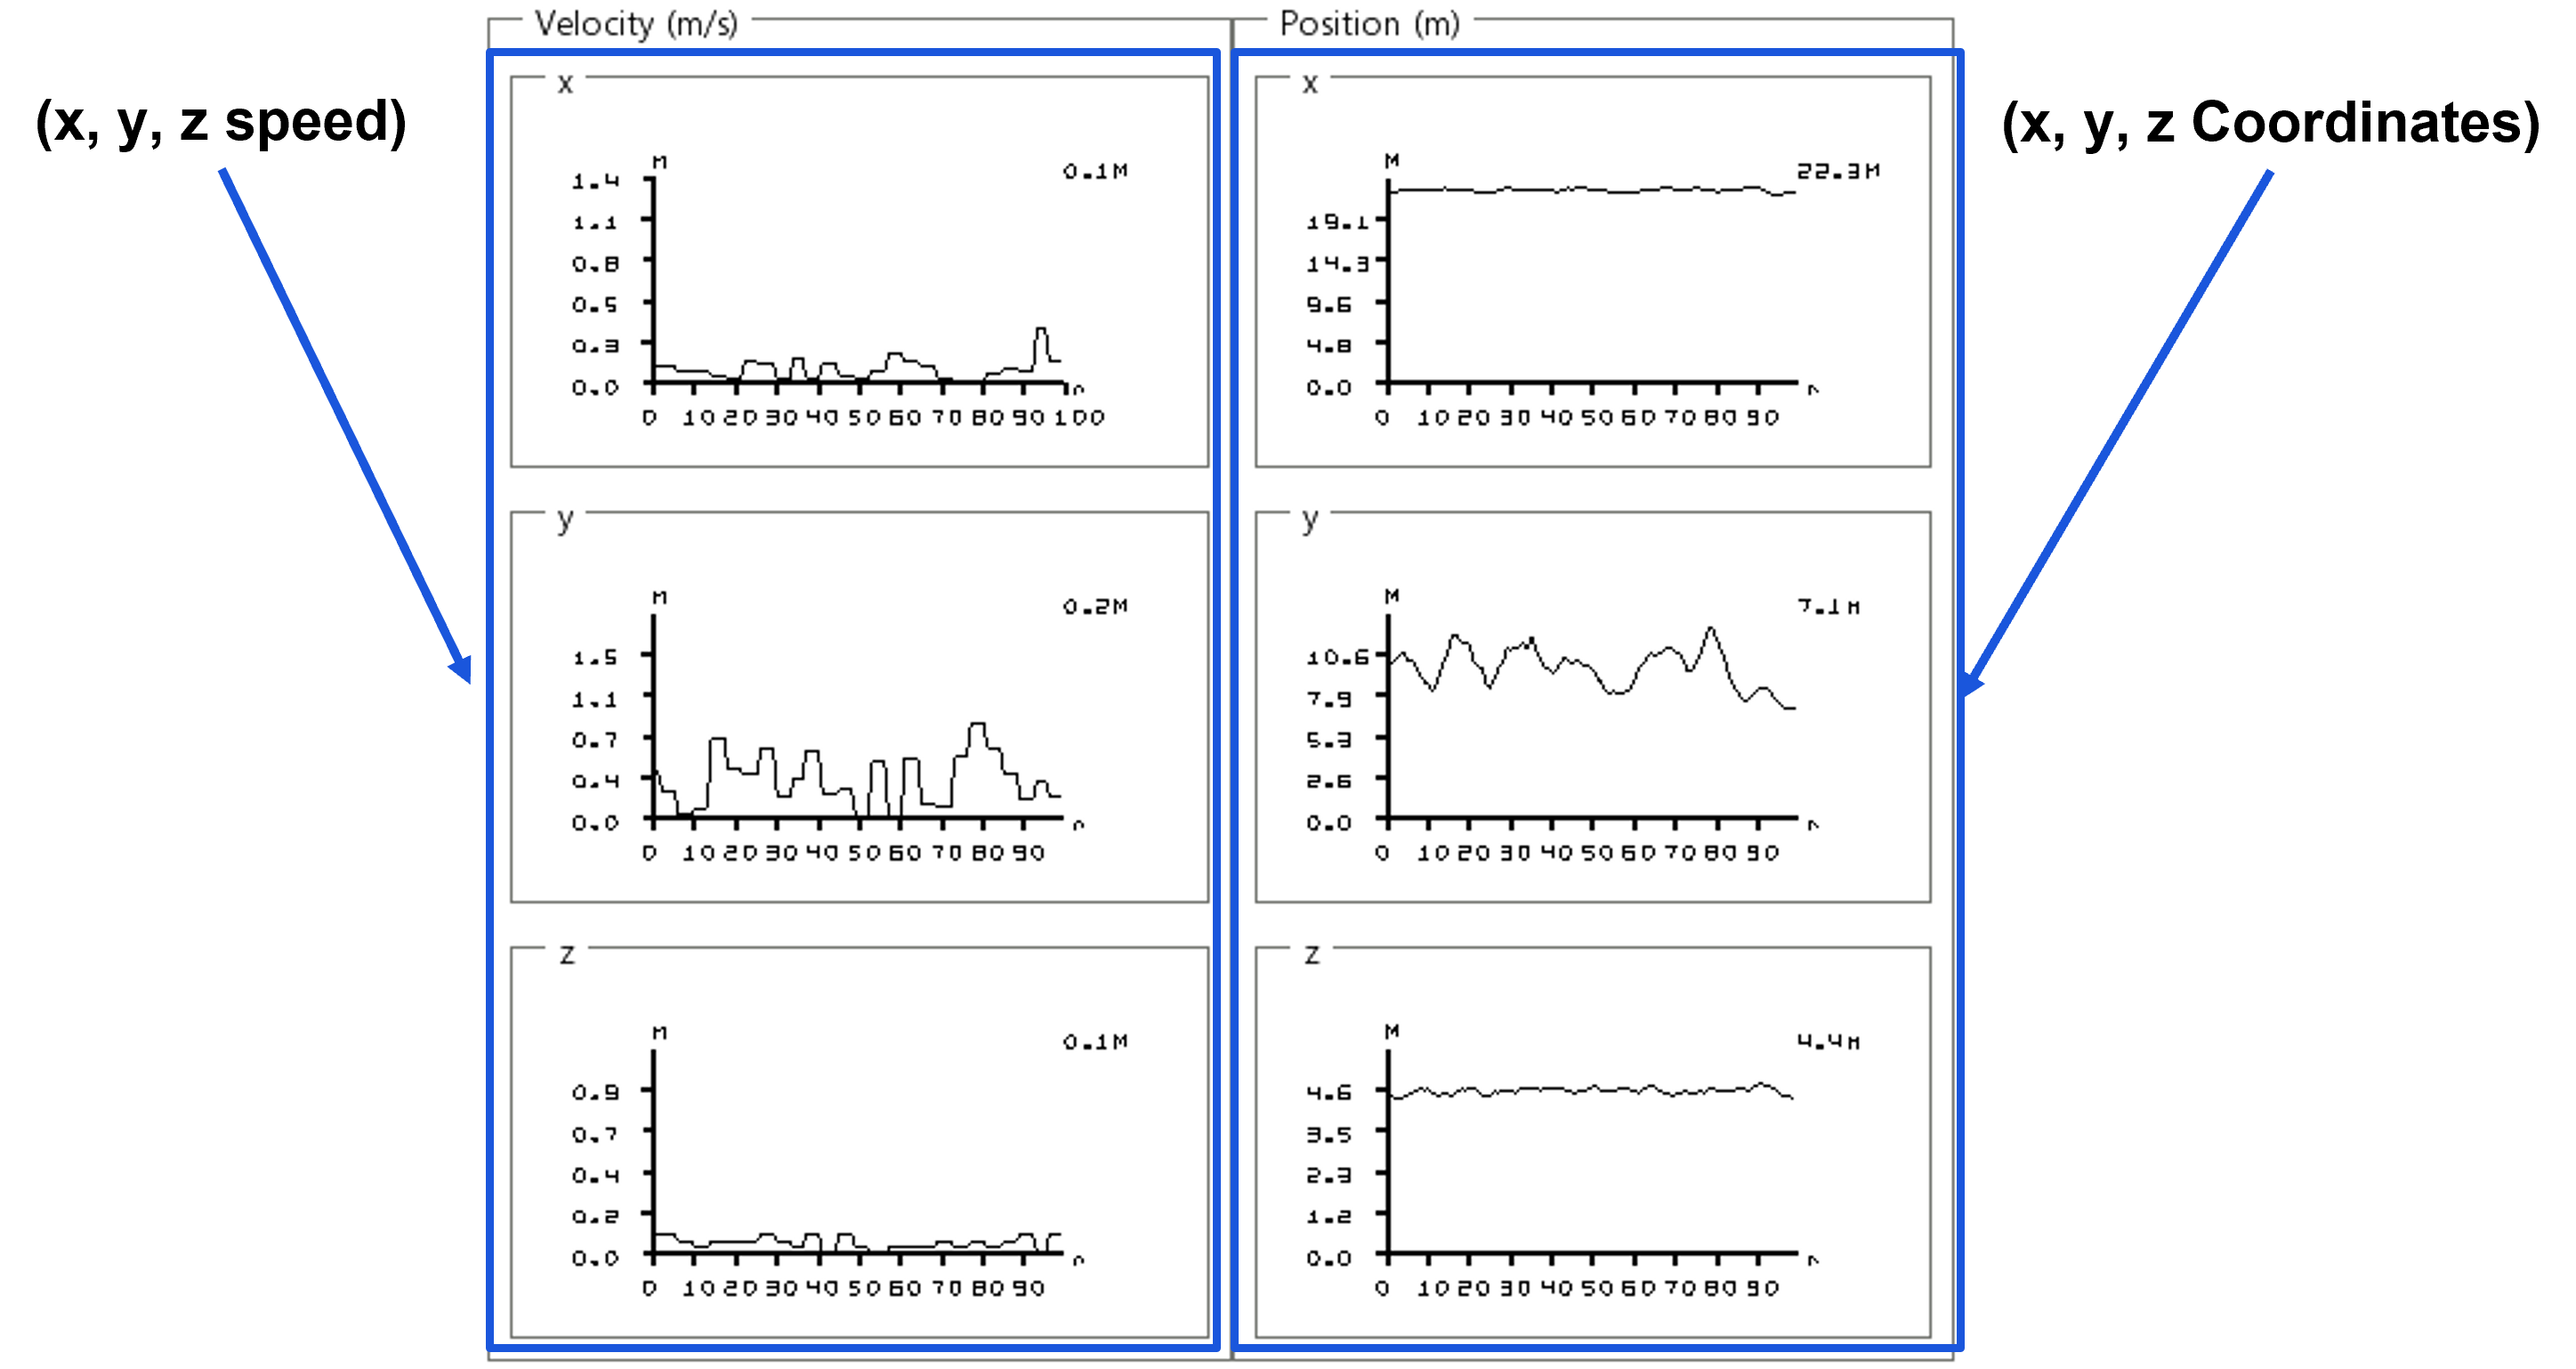
\includegraphics[width=1.0\columnwidth]{fig9.png}}
    \caption{Real-time speed and positioning visualization of tag movement.}
    \label{fig10}
\end{figure}


\subsection{Result analysis}
To evaluate the performance of the proposed clustering scheme, 1) no special technique is applied; 2) When only the clustering scheme is applied; 3) The clustering scheme and the minimum distance algorithm were divided into three cases.

The experiment was executed indoors during 10 minutes. As shown in Table \ref{tab1}, the average localization error was 46.3 cm as a result of the experiment using only trilateration. The average localization error in trilateration was reduced to 12.7 cm by applying the clustering scheme. Finally, it was confirmed that average localization error could be reduced to 10.2cm by combining the minimum distance algorithm with the clustering scheme.

As a result of the experiment, the proposed clustering scheme is a significant result in that it can greatly reduce the localization error in an indoor environment due to an obstacle occurs.


\begin{table}[htbp]
    \caption{Average error on Indoor Localization.}
    \begin{center}
        \begin{tabular}{|c|c|c|c|}
            \hline
            \textbf{Measurement} & \multicolumn{3}{|c|}{\textbf{Standard error on 3 schemes}}                                                                       \\
            \cline{2-4}
            \textbf{Unit}        & \textbf{\textit{None}}                                     & \textbf{\textit{Clustering}} & \textbf{\textit{+ Minimum distance}} \\
            \hline
            cm                   & 46.3                                                       & 12.7                         & 10.2                                 \\
            \hline
        \end{tabular}
        \label{tab1}
    \end{center}
\end{table}


\section{Conclusion}

In this paper, a real-time clustering scheme was proposed to reduce the localization error of 3D indoor localization using a wireless anchors. In addition, to evaluate the performance of the proposed scheme, a test bed for performance experiment was developed and constructed. As a result of the experiment, it was confirmed that the proposed clustering scheme can significantly reduce the localization error in an indoor environment due to an obstacle environments.

Based on this study in the future, we plan to further improve the localization performance of the proposed scheme with multi-tag environment in 3D indoor localization.

\section*{Acknowledgments}

This research was supported by the BB21plus funded by Busan Metropolitan City and Busan Institute for Talent \& Lifelong Education (BIT).

This work was supported by the National Research Foundation of Korea (NRF) grant funded by the Korea government (MSIT) (No. 2019R1F1A1062670).

\begin{thebibliography}{00}
    \bibitem{b1} Park Jee Woong, Cho Yong K, Martinez, Diego, "A BIM and UWB Integrated Mobile Robot Navigation System for Indoor Position Tracking Applications," 6(2), pp.30-39, 2016.
    \bibitem{b2} J. Maneesilp, C. Wang, H. Wu and N. Tzeng, "RFID Support for Accurate 3D Localization," in IEEE Transactions on Computers, vol. 62, no. 7, doi: 10.1109/TC.2012.83, pp.1447-1459, July 2013.
    \bibitem{b3} M. Yoon, M. Kim and C. Lee, "A Dynamic Cell Clustering Algorithm for Maximization of Coordination Gain in Uplink Coordinated System," in IEEE Transactions on Vehicular Technology, vol. 65, no. 3, doi: 10.1109/TVT.2015.2413899, pp.1752-1760, March 2016.
    \bibitem{b4} Y. K. Cho and J. Youn, “Wireless Sensor-driven Intelligent Navigation Robots for Indoor Construction Site Security and Safety,” in 23rd ISARC, pp.493–498, 2006.
    \bibitem{b5} J. Park, Y. K. Cho, and C. Ahn, “Wireless Tracking System Integrated with BIM for Indoor Construction Applications,” in Proceedings of the 2016 Construction Research Congress (CRC), 2016.
    \bibitem{b6} F. Subhan, H. Hasbullah, and K. Ashraf, "Kalman filter-based Hybrid Indoor Position Estimation Technique in Bluetooth Networks," Int. J. Navig. Obs. 2013.
    \bibitem{b7} K. Kim and Y. Cho, "BIM-Based Planning of Temporary Structures for Construction Safety," Comput. Civ. Eng. 2015.
    \bibitem{b8} X. Guo, Z. Chen, X. Hu and X. Li, "Multi-Source Localization Using Time of Arrival Self-Clustering Method in Wireless Sensor Networks," in IEEE Access, vol. 7, pp. 82110-82121, 2019.
\end{thebibliography}

\end{document}
